\chapter{Testování a nasazení}

\section{Testování}
V této sekci jsou popsány způsoby, jakými byla aplikace testována. K testování bylo využito jak metodik statické analýzy kvality kódu, tak i automatické testování pomocí jednotkových a integračních testů.

Statická analýza kvality kódu byla provedena nástrojem PHPSpec \autocite{phpspec}. Testování pomocí jednotkových a integračních testů bylo provedeno nástrojem PHPUnit \autocite{phpunit}.
Výstup testování pomocí PHPUnit se nachází v ukázce kódu \emph{\ref{phpunit-volani}}. 


\begin{listing}[htbp]
        \begin{minted}{console}
$ php vendor/bin/phpunit 
PHPUnit 6.2.2 by Sebastian Bergmann and contributors.

..................................................  50 / 121 ( 41%)
.................................................. 100 / 121 ( 82%)
.....................                              121 / 121 (100%)

Time: 41.4 seconds, Memory: 102.00MB

OK (121 tests, 191 assertions)
        \end{minted}
    \caption{Výstup PHPUnit testů \label{phpunit-volani}}
\end{listing}

 

 

\subsection{Pokrytí kódu testy}
Na obrázku \emph{\ref{phpunit-coverage}} je možné vidět pokrytí kódu testy, vygenerované pomocí PHPUnit.

\begin{figure}[htbp]
    \centering
    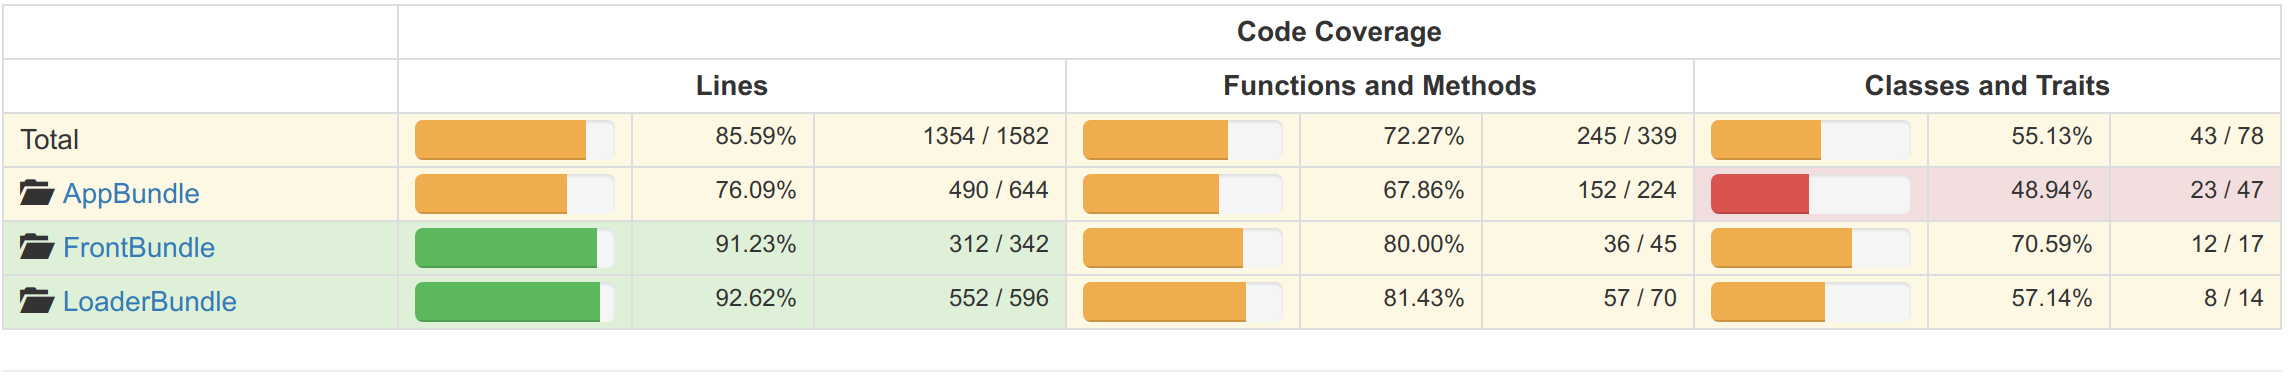
\includegraphics[width=\textwidth,height=\textheight,keepaspectratio]{images/coverage.png}
    \caption{Pokrytí kódu testy\label{phpunit-coverage}}
\end{figure}


\section{Nasazení}
Aplikace byla nasazena na školní \gls{VPS}, který byl speciálně zřízen pro potřeby mé aplikace. Na serveru běží operační systém CentOS 7 \autocite{centos}. Vzhedem k tomu, že jsem obdržel administrátorská práva k systému, bylo možné nainstalovat všechny potřebné závislosti, kterých aplikace využívá. 

Při instalaci bylo postupováno podle instalační příručky (příloha \emph{\ref{append:instalace}}), včetně úspešného běhu testů. 

Aplikace je nasazena a připravena k~používání na adrese \url{http://printabrick.org}. 


